\documentclass[]{article}
\usepackage{mathrsfs}
\usepackage{amsmath}
\usepackage{amsfonts}
\usepackage{graphicx}
\usepackage[left=20mm, right=20mm, top=20mm, bottom=20mm]{geometry}
\begin{document}

\Huge Series y transformada de Fourier
\normalsize
\\

En este apunte se propone estudiar las series y la transformada de Fourier, para ello primero veremos algunos conceptos sobre señales y sistemas.
\\
El concepto de señal es muy utilizado en diversas áreas de la ciencia y la tecnología como las comunicaciones, el diseño de circuitos, la acústica, control de procesos quimicos, etc. Lo que caracteriza a todas las señales eas ser una magnitud física que varía con el tiempo y que lleva información generalmente acerca del estado o comportamiento de un sistema. Los sistemas reciben señales de entrada y producen señales de salida, veremos mas acerca de esto en la unidad de Sistemas estables.
Clasificaremos a las señales de acuerdo a la variable independiente, diremos de tiempo continuo o de tiempo discreto.\\
Las señales de tiempo continuo son muy utiles para realizar modelos matematicos de fenomenos físicos como los circuitos electricos o las comunicaciones.\\
Las señales de tiempo discreto son muy utiles para el análisis numerico, la estadística y el análisis de datos economicos o demográficos.\\
\\
\large Señales digitales
\normalsize
\\
Una señal digital es aquella que presenta una variación discontinua y que solo puede tomar ciertos valores discretos. Matematicamente podemos decir que el conjunto imagen de la función que describe esta señal es finito.
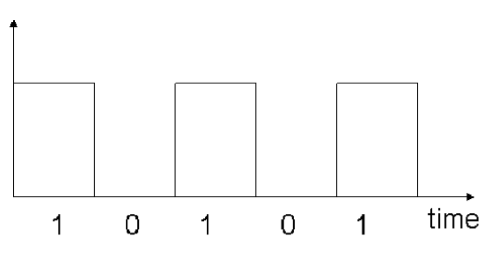
\includegraphics{../../../Imagenes/Superior/Fourier/Fourier01.PNG}

\large Señal analógica
\normalsize
\\
Una señal analógica es aquella que presenta una variación	continua con el tiempo, es decir, son señales que varían en forma suave. Matematicamente podemos decir que el conjunto imagen de la funcion que describe esta señal es continuo.

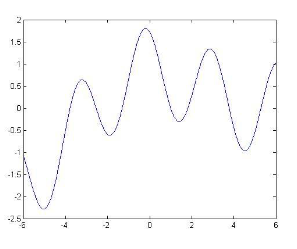
\includegraphics{../../../Imagenes/Superior/Fourier/Fourier02.PNG}
\\
\\
\huge Series de Fourier
\normalsize
\\

En 1807, Fourier demostró que casi toda función periódica se puede representar mediante una sumatoria de senos y cosenos. Dicha expresión de una función se conoce como la Serie de Fourier. A continuación presentaré las formulas necesesarias y nos preocuparemos por su interpretación mas adelante. Se recomienda fuertemente buscar la demostración de estas formulas ya que no se presentarán aqui pues estas suponen una buena base de algebra lineal y geometría analítica además de un pensamiento muy abstracto sobre espacios vectoriales de infinitas dimensiones. Para el propósito de la materia las tomaremos como ciertas.
\begin{align}
S(x)  &= \frac{a_0}{2} + \sum_{n=1}^{\infty} a_n \cos(n\omega x) +b_n\sin(n \omega x) \\
 a_n &= \frac{1}{L}\int_{-L}^{L}f(x)\cos(n\omega x)dx  \\
 b_n &=\frac{1}{L}\int_{-L}^{L}f(x)\sin(n\omega x)dx  \\
  L&= \frac{T}{2}
\end{align}

Teniendo en cuenta el desarrollo en Serie trigonometrica de Fourier, podemos considerar una señal digital como suma de señales analógicas.

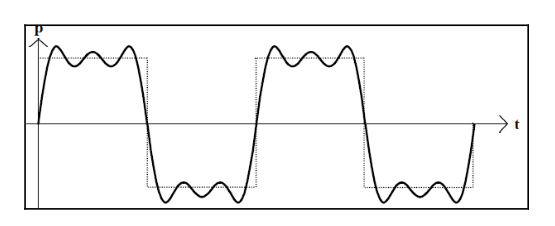
\includegraphics{../../../Imagenes/Superior/Fourier/Fourier03.PNG}

Empiezan las definiciones:\\
Dada una función seccionalmente continua en un intervalo $[a,b]$ desarrollarla en Serie de Fourier significa escribirla como combinación lineal de las funciones de una base ortonormal de funciones dada.
\\
\\
\large Función seccionalmente continua
\normalsize
\\
\\
Sea $f:[a,b]\rightarrow \mathbb{R}$ Se dice que $f$ es seccionalmente continua $\Leftrightarrow$ tiene un numero finito de saltos finitos. También se llama continua a trozos.

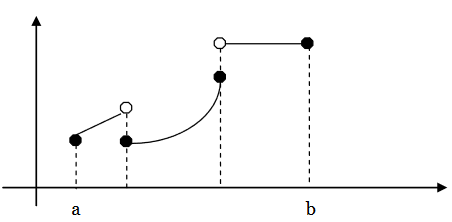
\includegraphics{../../../Imagenes/Superior/Fourier/Fourier04.PNG}

Toda funcion $f$ seccionalmente continua en $[a,b]$ es integrable  en $[a,b]$, es decir, existe la integral y es convergente $\int_{a}^{b}f(x)dx$
\\
\\
\Large Serie trigonometrica de Fourier
\normalsize
\\
\\
La serie trigonometrica de Fourier, es un caso particular de las Series de Fourier, en la cual se toma como base ortonormal en $[0,2\pi]$, con $n\in \mathbb{N}$:
$$
B=(\frac{1}{\sqrt{2\pi}};\frac{\cos(nx)}{\sqrt{\pi}};\frac{\sin(nx)}{\sqrt{\pi}})
$$
\\
Como la base tiene infinitos vectores (funciones), el espacio vectorial es de dinmensión infinita.
\\
Veremos un ejemplo:
\\
Sea 
$$
f(x) = \left\{
	\begin{array}{ll}
		-\frac{\pi}{4}&  -\pi < x < 0 \\
		\frac{\pi}{4}& 0 < x < \pi \\
	\end{array}
\right. \hspace{10pt} \wedge \hspace{10pt} f(x) = f(x+2\pi)
$$
\\
Primero graficamos la función.

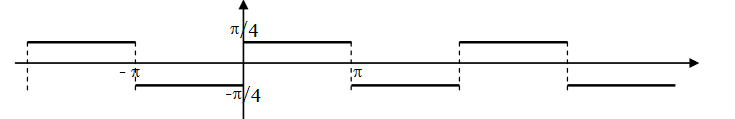
\includegraphics{../../../Imagenes/Superior/Fourier/Fourier05.PNG}

Ahora calculamos los coeficientes con las formulas: 
$$
a_0 = \frac{1}{\pi} \int_{-\pi}^{\pi}f(x)dx = 0
$$
$$
a_n = \frac{1}{\pi} \int_{-\pi}^{\pi}f(x)\cos(nx)dx = 0
$$
No es necesario realizar las integrales para llegar a esta conclusión pero luego veremos como se justifica.\\
Para los $b_n$ sí es necesario realizar el cálculo integral:
$$
b_n = \frac{1}{\pi} \int_{-\pi}^{\pi}f(x)\sin(nx)dx = \frac{1}{2n}(1-(-1)^{n})
$$
No entraremos en detalles de las cuentas, pero pueden verificarlo por ustedes mismos.\\
Notemos que si $n$ es par $\Leftrightarrow b_n=0$ y si $n$ es impar $\Leftrightarrow b_n = \frac{1}{n}$ Por esto, en la fomula de la serie reemplazamos $n$ con $2k+1$:
$$
S(x) = \sum_{k=0}^{\infty}\frac{1}{2k+1}\sin[(2k+1)x]
$$
Y así queda desarrollada la función en series de Fourier. Si vemos el grafico de la sumatoria vemos que a medida que crece $k$ el grafico se acerca al de la función original.








\end{document}